\chapter{Results and Analysis} \label{Chap4}

\section{Main Results: Overall Performance under Two Reward Conditions}

\begin{table}[h]
\centering
\begin{tabular}{lccccc}
\hline
Metric & Baseline & PPO (Misaligned) & GRPO (Misaligned) & PPO (Sparse) & GRPO (Sparse) \\
\hline
Success rate & 5.0\% & 0.0\% $\pm$ 0.0\% & 1.3\% $\pm$ 1.2\% & 0.3\% $\pm$ 0.6\% & 1.3\% $\pm$ 1.5\% \\
Mean return & 244.0 & 431.4 $\pm$ 8.0 & 210.5 $\pm$ 9.1 & 183.6 $\pm$ 56.5 & 193.6 $\pm$ 6.5 \\
\hline
\end{tabular}
\caption{Overall performance under two reward conditions. The PPO/GRPO entries report the cross-seed mean $\pm$ cross-seed std over the 3 training seeds (42, 98, 5075), each evaluated over 100 episodes; the Baseline is a single pretrained model, whose values are the mean over its 100 evaluation episodes.}
\label{tab:main}
\end{table}

\textbf{Misaligned Reward condition.} PPO's return soars to 431 on all 3 seeds, a 77\% increase over the baseline, yet the success rate consistently drops to 0\%, fully decoupling the return increase from task completion. This is the defining signature of reward hacking: PPO learns to maximize return rather than to complete the task. GRPO's return is stable at 211, only 13\% below the baseline, and it does not over-respond to this unreliable reward signal.

\textbf{Sparse Reward condition.} After removing the dense reward, PPO's behaviour diverges sharply across training seeds: seed 42's return collapses to 118, 52\% below the baseline, while seeds 98 and 5075 barely maintain 214--219, giving a cross-seed std as high as 56.5. Its behaviour is dominated by training stochasticity rather than task structure, indicating that PPO cannot obtain a stable learning signal under sparse rewards. GRPO's return is stable at 188--201 across all seeds, with a cross-seed mean of 194, without the collapse or seed divergence seen for PPO.

The cross-condition comparison shows that PPO's return drops from 431 (Misaligned) to 184 (Sparse), while GRPO drops only slightly from 211 to 194. The key implication is that GRPO is not locked into reward-hacking behaviour under the Misaligned condition, so it does not need to recover when the reward structure switches; whereas PPO's failure mode switches with the condition: hacking when the reward is misleading, and collapsing or stalling when the reward is sparse. The three seeds and the two conditions corroborate each other, indicating that these differences are systematic algorithmic-mechanism behaviours rather than accidental artifacts of individual seeds.

From a worst-case-seed perspective, the difference is equally pronounced: PPO's lowest return under the Sparse condition is 118.4, 52\% below the baseline, while GRPO's lowest is 188.1, only 23\% below; under the Misaligned condition every GRPO seed has a return of at least 200.9, whereas all three PPO seeds achieve a 0\% success rate despite high returns. In terms of the worst-case lower bound of fine-tuned performance, GRPO is significantly better than PPO, which is the direct basis for its being a safer fine-tuning option.

To rule out the influence of the checkpoint-selection metric on our conclusions, we additionally run a set of experiments using the success rate rather than the mean reward as the model-selection criterion, with all other settings identical to Section~3.3. The main results are:

\begin{table}[h]
\centering
\begin{tabular}{lccccc}
\hline
Metric & Baseline & PPO (Misaligned) & GRPO (Misaligned) & PPO (Sparse) & GRPO (Sparse) \\
\hline
Success rate & 5.0\% & 0.7\% $\pm$ 0.6\% & 1.7\% $\pm$ 2.1\% & 0.3\% $\pm$ 0.6\% & 1.3\% $\pm$ 1.5\% \\
Mean return & 244.0 & 431.2 $\pm$ 38.8 & 191.4 $\pm$ 28.9 & 183.6 $\pm$ 56.5 & 193.6 $\pm$ 6.5 \\
\hline
\end{tabular}
\caption{Results with success-rate-based checkpoint selection. Entries are cross-seed mean $\pm$ cross-seed std over the 3 training seeds; the Baseline is a single pretrained model.}
\label{tab:bysuccess}
\end{table}

Under the Sparse Reward condition, the checkpoints selected by success rate and by mean reward give identical results, a direct consequence of the two metrics being equivalent under a binary reward. Under the Misaligned Reward condition, even when the success rate is used as the criterion, PPO's return stays as high as 431, with seed 42's checkpoint reaching 476 yet a success rate of only 0.7\%, consistent with the low-success pattern under mean-reward selection. This shows that reward hacking is a systematic result of PPO's optimization process rather than an artifact of the checkpoint-selection metric. Under by-success selection GRPO's return is 191 and its success rate 1.7\%, remaining near the baseline and showing no reward hacking. Overall, the main conclusions are robust to the checkpoint-selection metric: PPO's reward hacking and Sparse-condition instability, and GRPO's conservative stability, do not depend on the model-selection method.

\section{Diagnostic Analysis}

The main results show that PPO engages in reward hacking when rewards are unreliable, while GRPO remains stable. In this section we further localize the source of the difference through three dimensions of diagnostic analysis: reward decomposition, KL divergence, and parameter-space distance.

\subsection{Reward Decomposition}

\begin{figure}[h]
\centering
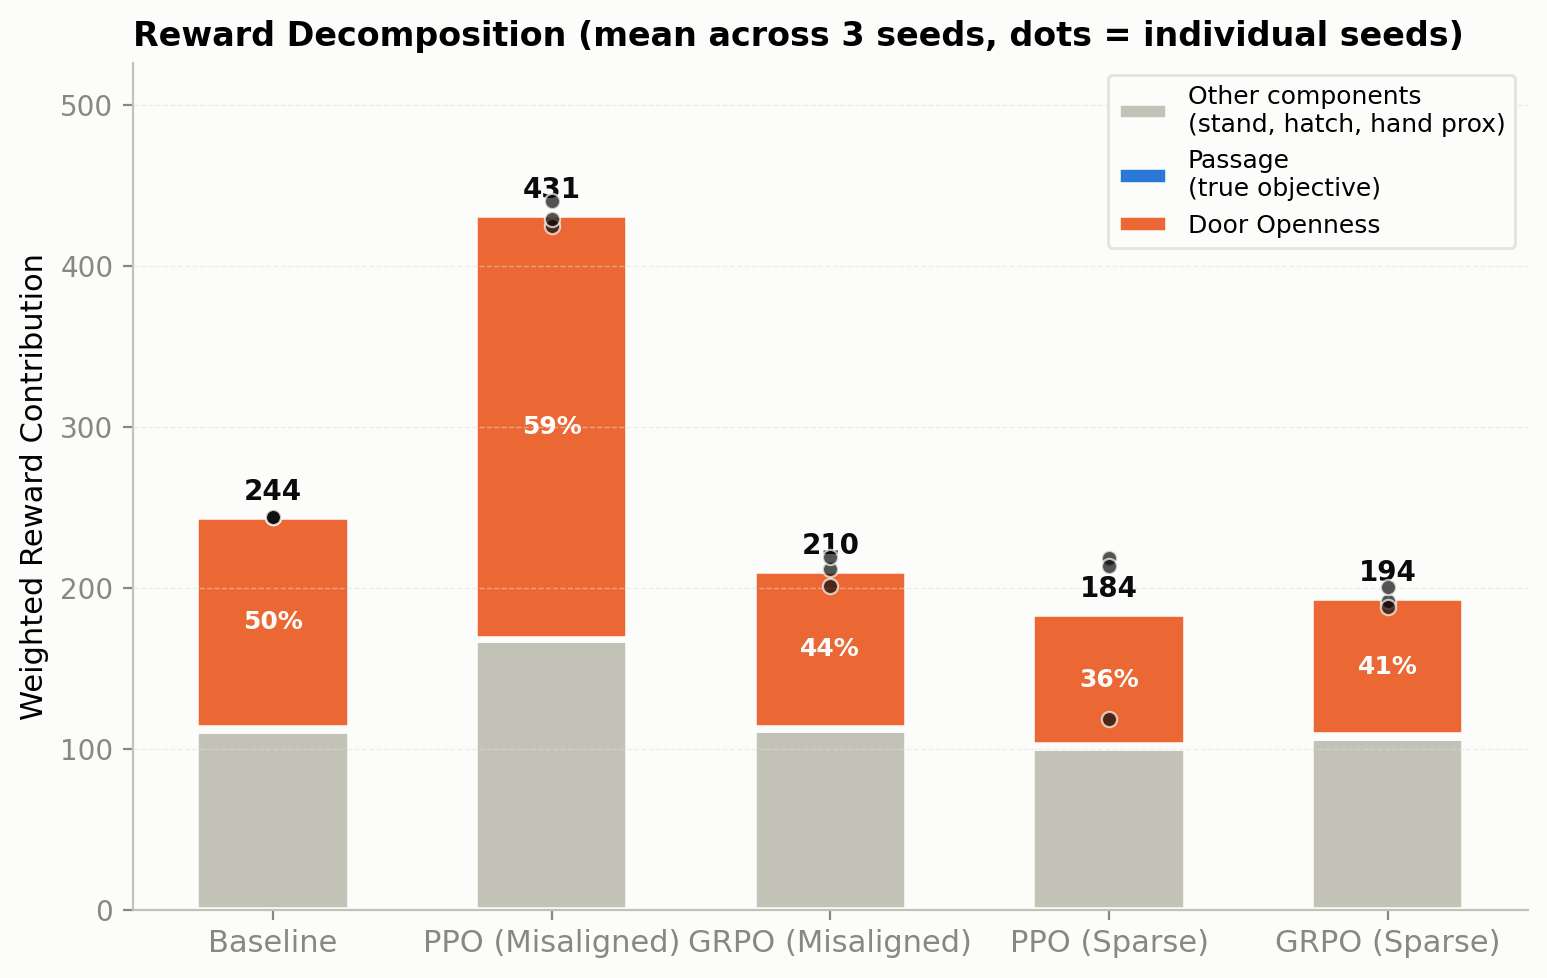
\includegraphics[width=0.8\textwidth]{../results/fig_reward_decomp.png}
\caption{Stacked-bar reward decomposition of each model on the Door task; the bar height is the accumulated value of each weighted component. Orange: door openness; blue: passing the door; grey: the remaining components.}
\label{fig:decomp}
\end{figure}

Comparison of the weighted contributions of each model (cross-seed mean $\pm$ cross-seed std over 3 seeds):

\begin{table}[h]
\centering
\begin{tabular}{lccccc}
\hline
Component (weight) & Baseline & PPO (Misaligned) & GRPO (Misaligned) & PPO (Sparse) & GRPO (Sparse) \\
\hline
Posture (0.1) & 61.6 $\pm$ 0.0 & 84.4 $\pm$ 1.3 & 61.3 $\pm$ 2.5 & 56.5 $\pm$ 3.8 & 59.0 $\pm$ 6.6 \\
Door openness (0.45) & 131.1 $\pm$ 0.0 & 263.4 $\pm$ 8.1 & 97.4 $\pm$ 8.4 & 81.2 $\pm$ 47.3 & 85.3 $\pm$ 16.7 \\
Handle press (0.05) & 17.7 $\pm$ 0.0 & 39.2 $\pm$ 0.4 & 18.2 $\pm$ 0.6 & 15.4 $\pm$ 4.0 & 17.5 $\pm$ 1.2 \\
Hand--handle dist. (0.05) & 32.0 $\pm$ 0.0 & 44.1 $\pm$ 0.5 & 31.8 $\pm$ 1.1 & 28.2 $\pm$ 4.2 & 30.4 $\pm$ 3.6 \\
Passing the door (0.35) & 1.7 $\pm$ 0.0 & 0.2 $\pm$ 0.1 & 1.8 $\pm$ 1.4 & 2.3 $\pm$ 2.5 & 1.4 $\pm$ 0.6 \\
\hline
\end{tabular}
\caption{Weighted component contributions (cross-seed mean $\pm$ cross-seed std over 3 seeds).}
\label{tab:components}
\end{table}

Change in the reward composition shares (cross-seed mean):

\begin{table}[h]
\centering
\begin{tabular}{lccccc}
\hline
Component & Baseline & PPO (Misaligned) & GRPO (Misaligned) & PPO (Sparse) & GRPO (Sparse) \\
\hline
Posture & 27.1\% & 21.1\% & 30.3\% & 37.0\% & 31.8\% \\
Door openness & 49.8\% & 58.5\% & 43.7\% & 35.9\% & 41.1\% \\
Handle press & 8.4\% & 9.4\% & 9.4\% & 8.8\% & 10.0\% \\
Hand--handle dist. & 14.2\% & 10.9\% & 15.7\% & 16.7\% & 16.4\% \\
Passing the door & 0.4\% & 0.1\% & 0.9\% & 1.6\% & 0.7\% \\
\hline
\end{tabular}
\caption{Reward composition shares (cross-seed mean, \%).}
\label{tab:shares}
\end{table}

Under the Misaligned condition, PPO's total reward increment over the baseline is $+187$ (cross-seed mean), of which the door-openness increment is $+294$ (unweighted), while the passing-the-door reward changes by $-4.1$; the door-openness share correspondingly rises from 49.8\% to 58.5\%, and the passing-the-door share falls from 0.4\% to 0.1\%. This shows that most of PPO's return gain comes from manipulating the door angle, while the reward that truly reflects task completion (passing the door) actually decreases, decoupling return growth from the task goal --- a typical reward-hacking signature. Notably, the amplification is not limited to door openness: posture rises from 61.6 to 84.4 and handle press from 17.7 to 39.2, both increasing significantly, with only the passing-the-door component decreasing. This indicates that PPO's hacking tendency is generic: any component that is available at every step and weakly related to the success condition is amplified. Door openness is amplified most strongly because its weight (0.45) is the highest, and because the door can be opened and closed repeatedly, giving a non-zero every-step reward with dense gradients, providing the largest return increment among equally accessible components; in contrast, the passing-the-door reward is near zero on the vast majority of trajectories and cannot provide effective gradients. This behaviour appears consistently across all seeds, with the cross-seed std of PPO's door\_openness being only 8.1. In contrast, GRPO (Misaligned)'s door-openness share (43.7\%) is even lower than the baseline, showing that it not only fails to amplify this component but relatively suppresses it; under the Sparse condition both models have shares below the baseline (PPO 35.9\%, GRPO 41.1\%), with no over-reliance on a single reward component. This also shows that whether reward hacking occurs depends on the algorithmic mechanism rather than on the reward weight structure itself.

\subsection{KL Divergence and Policy-Update Magnitude}

\begin{figure}[h]
\centering
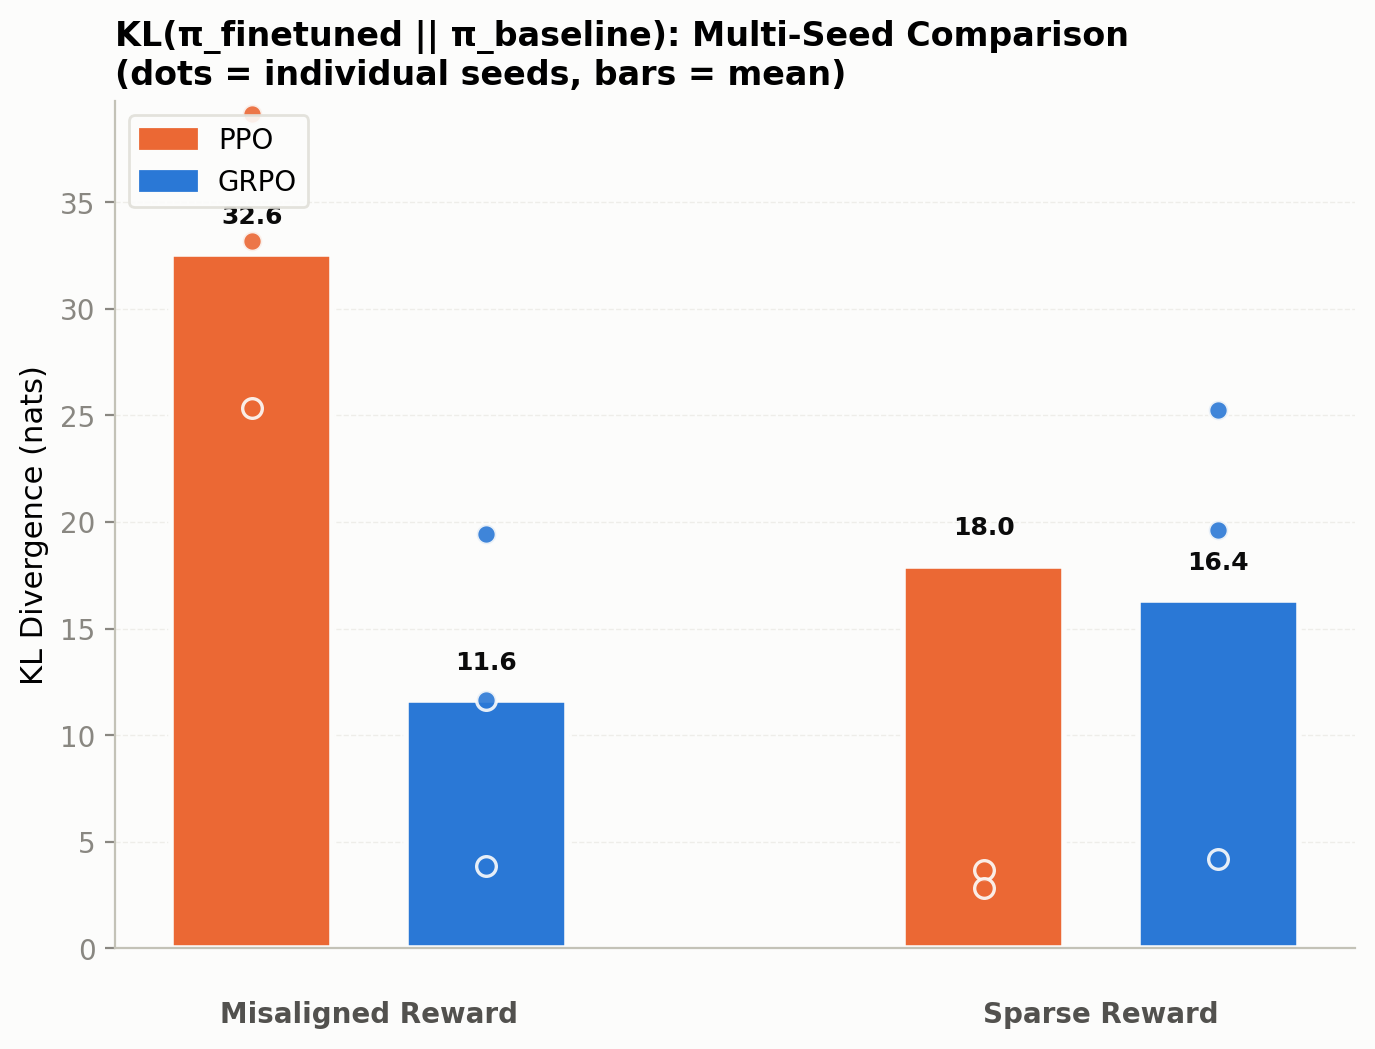
\includegraphics[width=0.8\textwidth]{../results/fig_kl_divergence.png}
\caption{Action-distribution KL divergence of each model relative to the Baseline, over 3 seeds; the bar height is the cross-seed mean and the dots are individual seeds.}
\label{fig:kl}
\end{figure}

On the same fixed 1000 observations collected by the baseline policy, we compute the KL divergence of each model's action distribution relative to the Baseline using the closed-form diagonal-Gaussian solution. The following table reports the cross-seed mean $\pm$ std over 3 seeds:

\begin{table}[h]
\centering
\begin{tabular}{lccc}
\hline
Model & Mean KL (nats) & Per-dim (nats/dim) & Per-seed \\
\hline
PPO (Misaligned) & 32.6 $\pm$ 6.9 & 0.53 & 25.4, 33.2, 39.2 \\
GRPO (Misaligned) & 11.6 $\pm$ 7.8 & 0.19 & 19.4, 11.7, 3.8 \\
PPO (Sparse) & 18.0 $\pm$ 25.5 & 0.29 & 47.4, 3.7, 2.8 \\
GRPO (Sparse) & 16.4 $\pm$ 10.9 & 0.27 & 19.6, 4.2, 25.2 \\
\hline
\end{tabular}
\caption{KL divergence of each model relative to the Baseline (cross-seed mean $\pm$ cross-seed std).}
\label{tab:kl}
\end{table}

In terms of update magnitude, all fine-tuned models have KL significantly greater than zero relative to the Baseline, the minimum being 2.8 nats, which is about 0.05 nats per dimension averaged over the 61-dimensional action space, showing that both types of policies undergo substantial updates and that GRPO's stability does not stem from policy stagnation. Under the Misaligned condition, PPO's update magnitude of 32.6 nats (0.53 per dimension) is about 3 times GRPO's 11.6 nats (0.19 per dimension), and all three seeds are consistently high at 25.4--39.2, corresponding to its reward-hacking behaviour; GRPO's update magnitude varies with seed in 3.8--19.4, but this variation does not translate into return fluctuation, reflecting KL-return decoupling. Under the Sparse condition, PPO's update magnitude diverges sharply across seeds: seed 42's KL explodes to 47.4 with a return collapse, while seeds 98/5075's KL collapses to 2.8--3.7 with policy stalling; GRPO's KL stays at 4.2--25.2 without collapse. Therefore, consistently across seeds and conditions, we observe that GRPO's update magnitude is variable but its return is stable, while PPO's update magnitude and return are tightly coupled and its failure mode switches with the condition.

\begin{figure}[h]
\centering
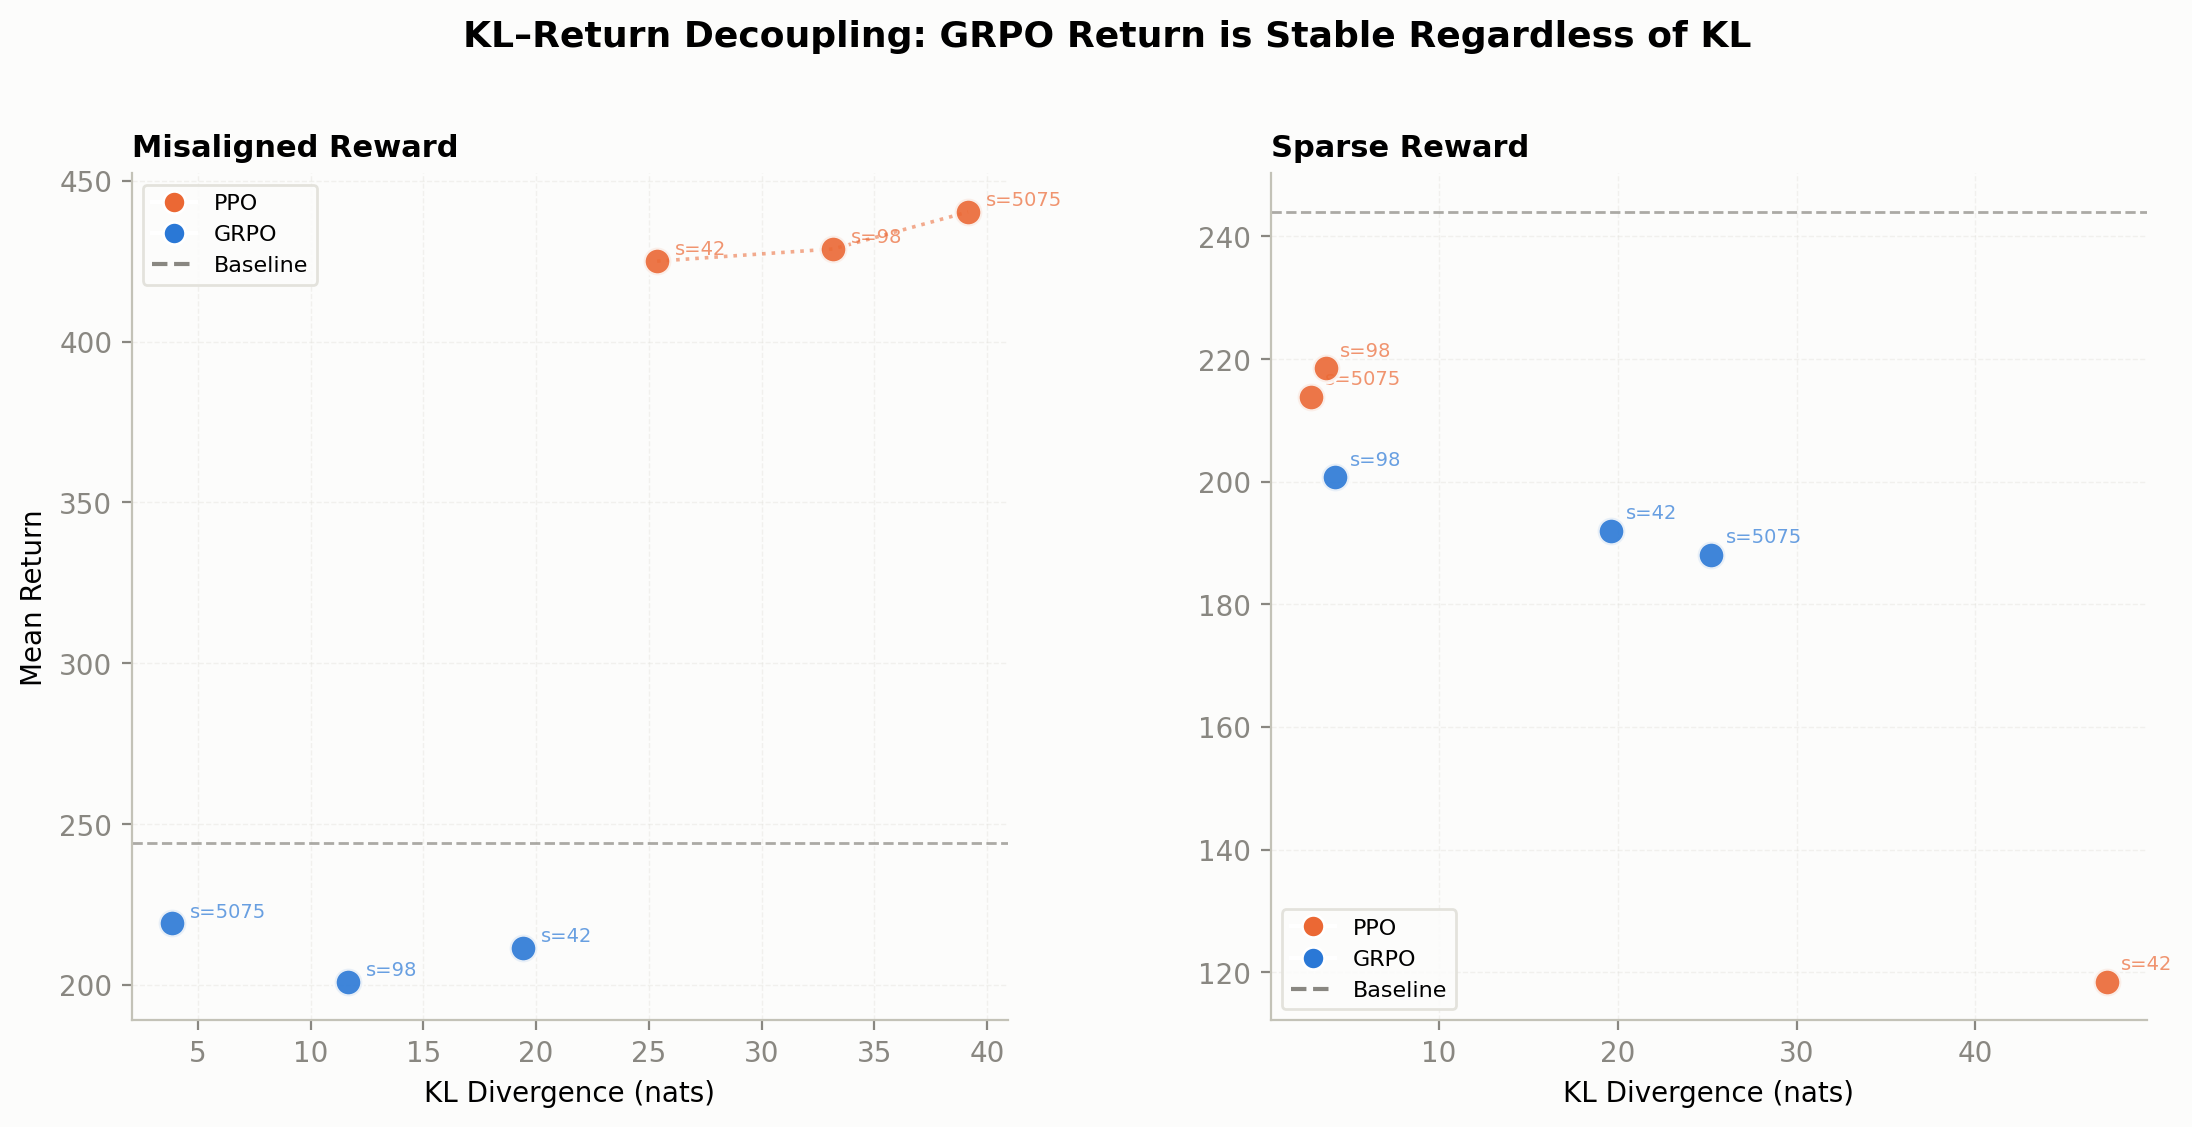
\includegraphics[width=0.8\textwidth]{../results/fig_kl_vs_return.png}
\caption{Scatter plot of KL divergence versus return, two panels, left = Misaligned Reward condition, right = Sparse Reward condition; the dashed line is the baseline reference.}
\label{fig:klvsreturn}
\end{figure}

Figure~\ref{fig:klvsreturn} shows GRPO's KL-return decoupling: under both conditions, GRPO's points cluster in a horizontal band around $return \approx 200$, with KL ranging from 3.8 to 25.2 while the return stays fixed; PPO behaves oppositely, with KL and return rising in tandem under the Misaligned condition and polarizing under the Sparse condition, where high KL corresponds to collapse and low KL to stalling. This contrast shows that GRPO's policy-update magnitude can vary with seed and condition, but the update direction always stays aligned with the task goal without reward hacking; PPO's update magnitude and direction are both driven by the reward signal and can easily become uncontrolled under unreliable rewards. Quantitatively, under the Sparse condition PPO's cross-seed KL bandwidth of 44.6 nats corresponds to a return bandwidth of 100.1, while GRPO's KL bandwidth of 21.0 nats corresponds to a return bandwidth of only 12.6: the seed-to-seed difference in update magnitude hardly propagates to GRPO's performance difference, yet significantly propagates to PPO's performance difference.

\begin{figure}[h]
\centering
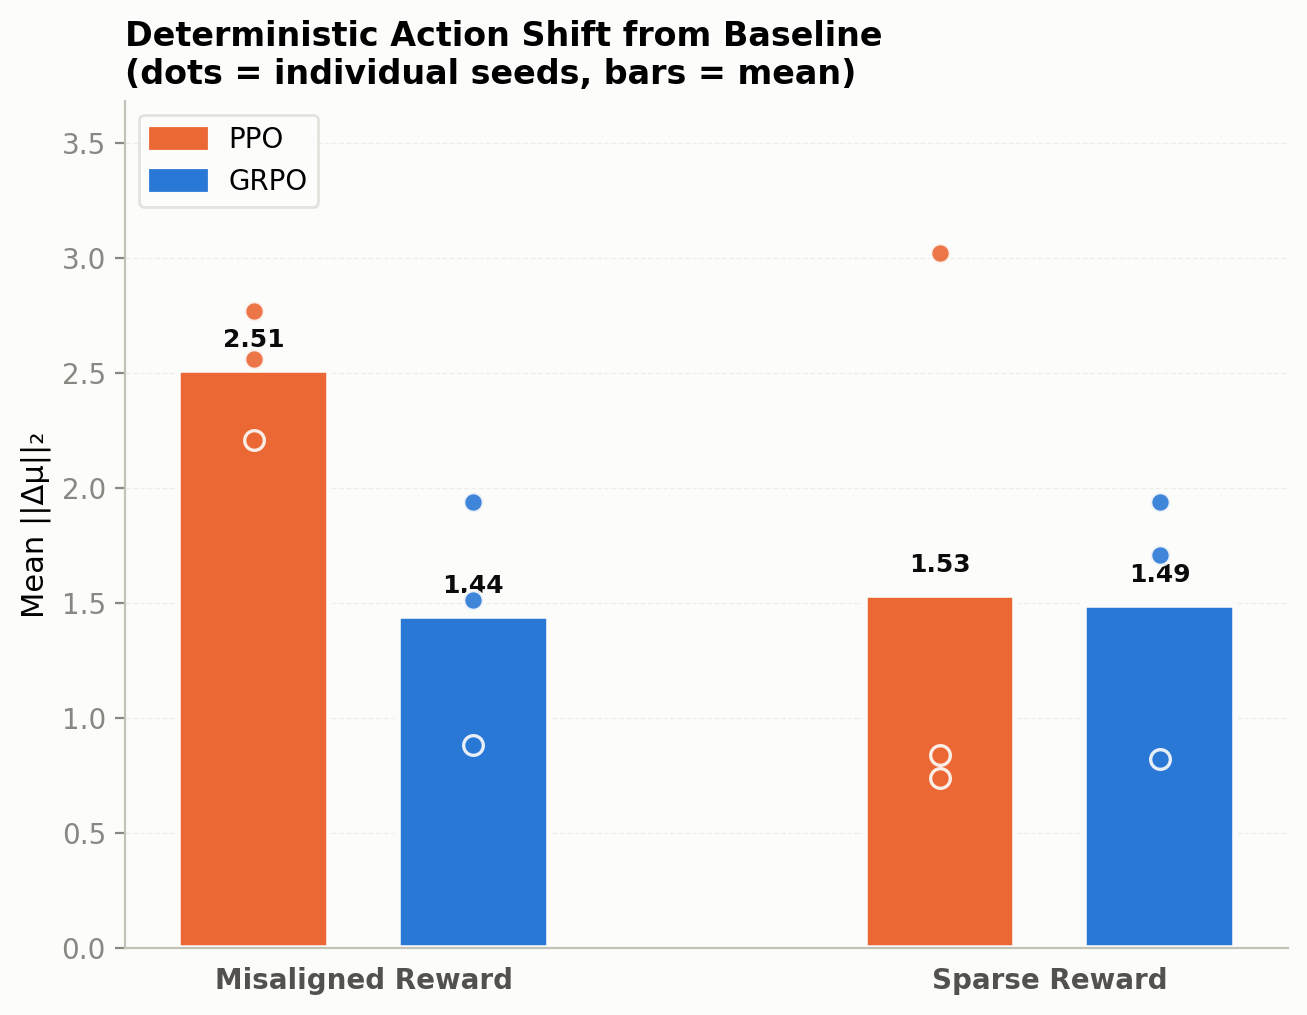
\includegraphics[width=0.8\textwidth]{../results/fig_action_diff.png}
\caption{L2 distance of each model's deterministic action mean relative to the Baseline, cross-seed mean, with dots for individual seeds.}
\label{fig:actiondiff}
\end{figure}

The cross-seed std of PPO (Sparse)'s action offset reaches 1.30, far higher than the other configurations; GRPO's action-offset means under the two conditions are 1.44 and 1.49 respectively, almost identical.

\begin{figure}[h]
\centering
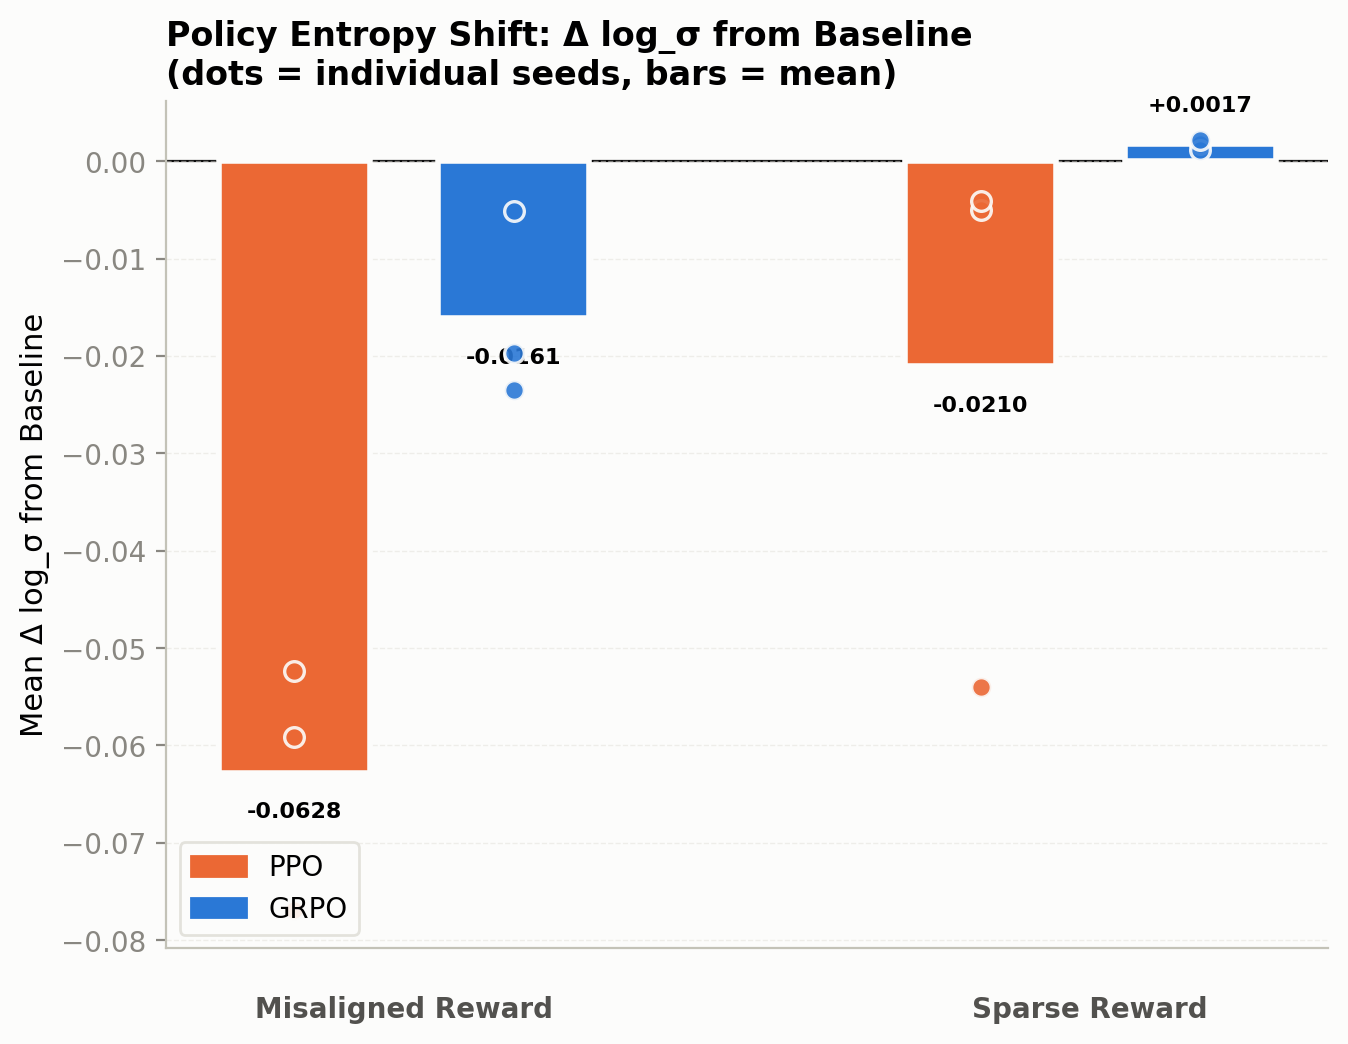
\includegraphics[width=0.8\textwidth]{../results/fig_logstd_shift.png}
\caption{Average log-$\sigma$ shift of each model relative to the Baseline, cross-seed mean, with dots for individual seeds.}
\label{fig:logstd}
\end{figure}

PPO (Misaligned) consistently reduces entropy across all seeds, with a shift of $-0.05$ to $-0.08$; this is one of the signatures of reward-hacking strategies: locking into a specific action pattern and reducing exploration to sustain a high return. PPO (Sparse)'s log-$\sigma$ change is highly inconsistent across seeds, with a cross-seed std of 0.028, consistent with its seed-to-seed return fluctuation. GRPO (Sparse)'s log-$\sigma$ is almost unchanged across the three seeds, with a shift of $+0.002 \pm 0.001$, maintaining the same exploration level as the Baseline; this may be a key factor enabling GRPO to avoid deterministic collapse under extremely sparse rewards.

\subsection{Parameter-Space Distance}

\begin{figure}[h]
\centering
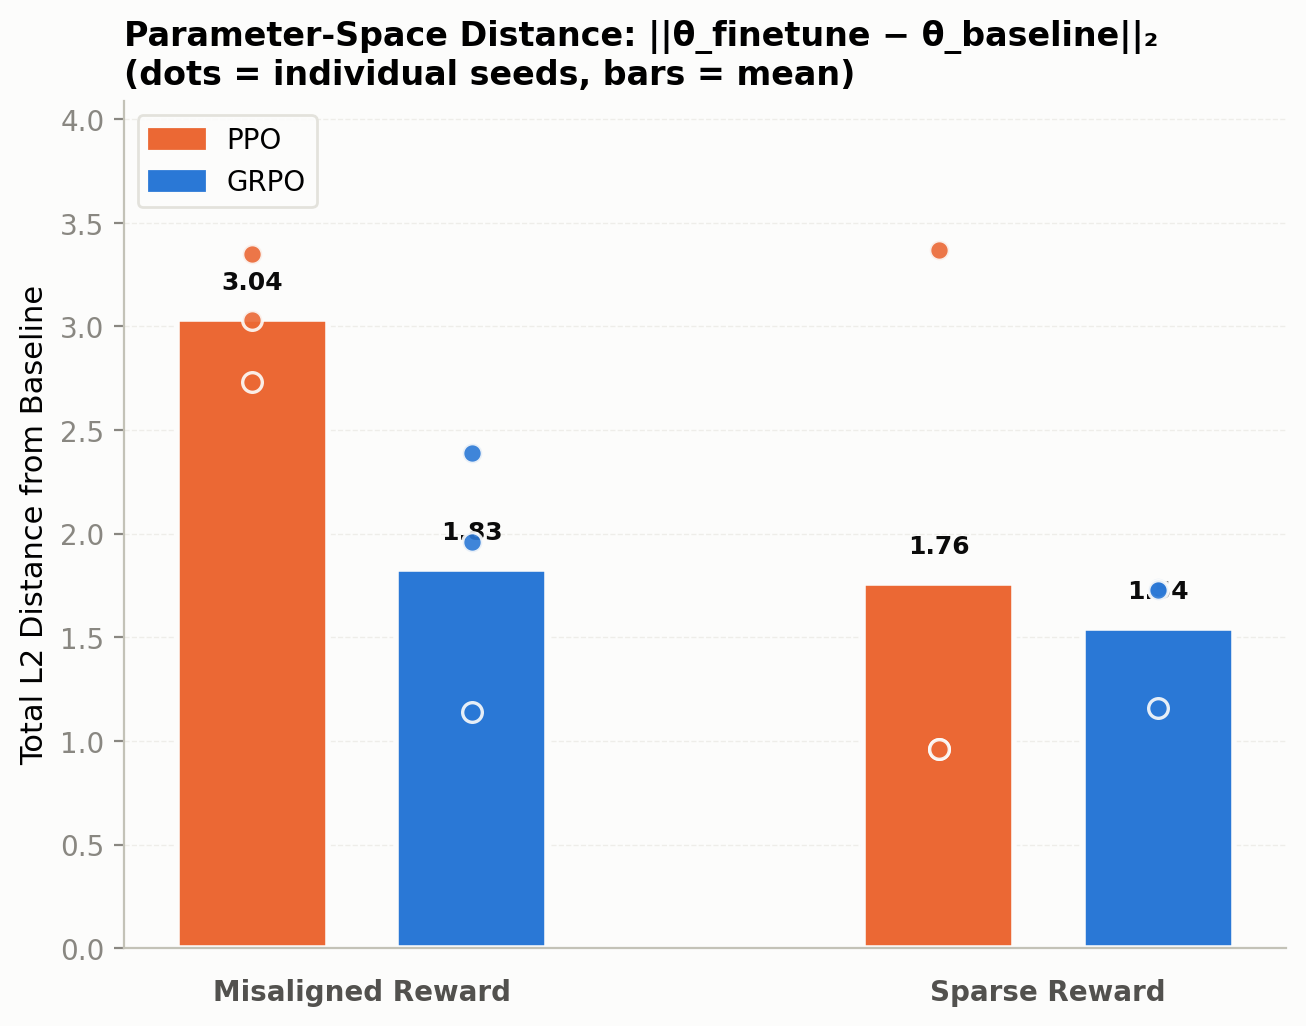
\includegraphics[width=0.8\textwidth]{../results/fig_param_distance.png}
\caption{Parameter-space L2 distance of each model relative to the Baseline, cross-seed mean, with dots for individual seeds.}
\label{fig:param}
\end{figure}

The cross-seed std of PPO (Sparse)'s parameter distance reaches 1.36; seed 42's parameter offset of 3.37 is about 3 times the 1.09/0.96 of seeds 98/5075. GRPO's parameter-distance means under the two conditions are 1.83 and 1.43. This cross-seed variation pattern is consistent with the action-distribution KL; for example, GRPO (Misaligned)'s KL std of 7.8 corresponds to a parameter-distance std of 0.63, the two metrics reflecting the same update characteristics from different levels.

\subsection{VecNormalize Drift}

\begin{table}[h]
\centering
\begin{tabular}{lcc}
\hline
Model & $\lVert \Delta \text{mean} \rVert$ & $\lVert \Delta \text{var} \rVert$ \\
\hline
PPO (Misaligned) & 0.24 $\pm$ 0.04 & 16.3 $\pm$ 3.5 \\
GRPO (Misaligned) & 0.19 $\pm$ 0.11 & 13.4 $\pm$ 8.3 \\
PPO (Sparse) & 0.24 $\pm$ 0.29 & 17.5 $\pm$ 22.1 \\
GRPO (Sparse) & 0.35 $\pm$ 0.18 & 24.3 $\pm$ 12.8 \\
\hline
\end{tabular}
\caption{VecNormalize observation-statistic drift (cross-seed mean $\pm$ cross-seed std).}
\label{tab:vecnorm}
\end{table}

The VecNormalize observation statistics drift as the policy distribution changes during training; it must be confirmed that this does not constitute an alternative explanation for the above conclusions. The drift magnitude across the four configurations is broadly similar: the cross-seed mean of $\lVert\Delta\text{mean}\rVert$ ranges over 0.19--0.35 and $\lVert\Delta\text{var}\rVert$ over 13--24, with only PPO (Sparse) having a higher cross-seed dispersion, with a cross-seed std of 22.1 for $\lVert\Delta\text{var}\rVert$. The drift does not exhibit a systematic pattern matching the KL or return differences, and does not change the conclusions of Sections~4.2.2--4.2.3.

\subsection{Summary}

The evidence across seeds points consistently to the following: PPO either reward-hacks, or collapses or stalls, when rewards are unreliable, and this behaviour is reproducible across seeds; GRPO, by contrast, has substantial policy updates while its return stays stable, i.e., KL-return decoupling. Multiple metrics at the level of the action distribution, the parameter space and the exploration level corroborate each other, and this contrast does not depend on the checkpoint-selection metric.

\section{Ablation Study: The Role of the KL Penalty}

The standard GRPO adds a KL penalty relative to a reference policy in its loss, whereas the GRPO in our main experiments follows Doorman's implementation and removes this penalty. To confirm that the stability is attributable to group-relative advantage rather than to the absence of the KL penalty, we add a GRPO ablation with the KL penalty, with coefficient $\beta=0.01$ and all other settings identical to the main experiments, covering the 3 training seeds and the two reward conditions. The results are:

\begin{table}[h]
\centering
\begin{tabular}{lcccc}
\hline
Metric & Baseline & GRPO & GRPO+KL & PPO \\
\hline
Return (Misaligned) & 244.0 & 210.5 $\pm$ 9.1 & 222.4 $\pm$ 16.4 & 431.4 $\pm$ 8.0 \\
Return (Sparse) & 244.0 & 193.6 $\pm$ 6.5 & 217.9 $\pm$ 15.5 & 183.6 $\pm$ 56.5 \\
door share (Misaligned) & 49.8\% & 43.7\% & 49.2\% & 58.5\% \\
door share (Sparse) & 49.8\% & 41.1\% & 48.3\% & 35.9\% \\
Success (Misaligned) & 5.0\% & 1.3\% $\pm$ 1.2\% & 3.0\% & 0.0\% $\pm$ 0.0\% \\
Success (Sparse) & 5.0\% & 1.3\% $\pm$ 1.5\% & 1.7\% & 0.3\% $\pm$ 0.6\% \\
\hline
\end{tabular}
\caption{KL-penalty ablation results. The GRPO+KL column reports single-seed mean values (returns, success rates, door shares) across 3 seeds.}
\label{tab:klablation}
\end{table}

The GRPO with the KL penalty does not reward-hack under either condition: the door-openness shares of 49.2\% (Misaligned) and 48.3\% (Sparse) are basically level with the baseline's 49.8\%, whereas PPO's corresponding shares are 58.5\% and 35.9\%; the returns of 222 and 218 are close to the baseline and no lower than the no-KL version (210 and 194); the success rates of 3.0\% and 1.7\% are no worse than the no-KL version. This shows that regardless of whether the KL penalty is present, GRPO does not amplify a single reward component, and that the stability stems from the group-relative advantage mechanism itself.

The actual role of the KL penalty is to tighten the update magnitude rather than to decide whether hacking occurs. The KL of GRPO+KL relative to the baseline is 3.5 nats and its parameter distance is 1.33, both clearly smaller than the no-KL version's 11.6 nats and 1.83, but still significantly greater than zero (0.06 nats per dimension), showing that its policy still has substantial updates rather than stagnation; its return under the Sparse condition is actually higher (218 vs.\ 194) and it does not fail to learn because of the KL constraint.

\section{Cross-Task Validation: The Reach Task}

To further verify the generality of the above conclusions, we run additional experiments on the Reach task of HumanoidBench (`h1hand-reach-v0`). The Reach task requires the H1 robot's left hand to reach a target position, using a sparse binary success reward exactly like the Door Sparse condition: intermediate steps give a reward of 0, and a reward of 1.0 is given only at episode termination if the hand--target distance is less than 0.05 m. Both PPO and GRPO are initialized from the same pretrained Reach model with the same hyperparameters, and trained for 2M steps on a single seed.

The Reach task's sparse reward is more extreme than Door's: Door's reward function still has a weighted structure of 6 components, whose values, although not aligned with success, provide implicit behavioural gradients; Reach's reward contains only a single terminal binary signal, with intermediate steps entirely zero. The results are:

\begin{table}[h]
\centering
\begin{tabular}{lcc}
\hline
Metric & PPO (Sparse) & GRPO (Sparse) \\
\hline
Success rate & 0.0\% & 1.0\% \\
Mean return & 418.1 $\pm$ 320.9 & 712.6 $\pm$ 232.3 \\
\hline
\end{tabular}
\caption{Results on the Reach task.}
\label{tab:reach}
\end{table}

Because the evaluation dimensions of the pretrained Reach model and the fine-tuned models are incompatible, we cannot directly quantify how much of the pretrained success rate the fine-tuning recovers; we therefore compare only the relative performance of the two fine-tuning strategies: GRPO's return mean is higher, about 70\% above PPO, with a smaller variance (from $\pm$321 down to $\pm$232), and it is the only model with at least one success across the 100 evaluation episodes. Under the extreme condition of purely sparse, no-intermediate-guidance rewards, GRPO's relative advantage remains reproducible, consistent with the conclusions on the Door task. This result also reveals the boundary of GRPO's robustness: when the reward signal completely lacks intermediate-state discrimination, the within-group normalization of group-relative advantage may degenerate into pure noise and GRPO also cannot learn effectively; nevertheless, its performance still surpasses PPO.
